\definecolor{cfwone}{HTML}{eef5fa}
\definecolor{cfwtwo}{HTML}{daeaf5}
\definecolor{cfwthree}{HTML}{b2d2e9}
\definecolor{cfwfour}{HTML}{8abbde}

\newcommand{\fwone}[1]{\colbox{cfwone}{#1}\xspace}
\newcommand{\fwtwo}[1]{\colbox{cfwtwo}{#1}\xspace}
\newcommand{\fwthree}[1]{\colbox{cfwthree}{#1}\xspace}
\newcommand{\fwfour}[1]{\colbox{cfwfour}{#1}\xspace}

\newcommand{\fexp}[2]{\texttt{[{\color{darkgray}{#1:#2}}]}\xspace}
\newcommand{\fexptag}[1]{\fexp{TAG}{#1}}
\newcommand{\fexpfrom}[1]{\fexp{FROM}{#1}}
\newcommand{\fexpto}[1]{\fexp{TO}{#1}}
\newcommand{\fexptemp}[1]{\fexp{TEMP}{#1}}


\section{Use 3: Counterfactual Explanations}
\label{sec:app_explain}
%Both counterfactual explanations and semi-counterfactual explanations.
%As defined in \cite{}







\begin{figure}[t]
\centering
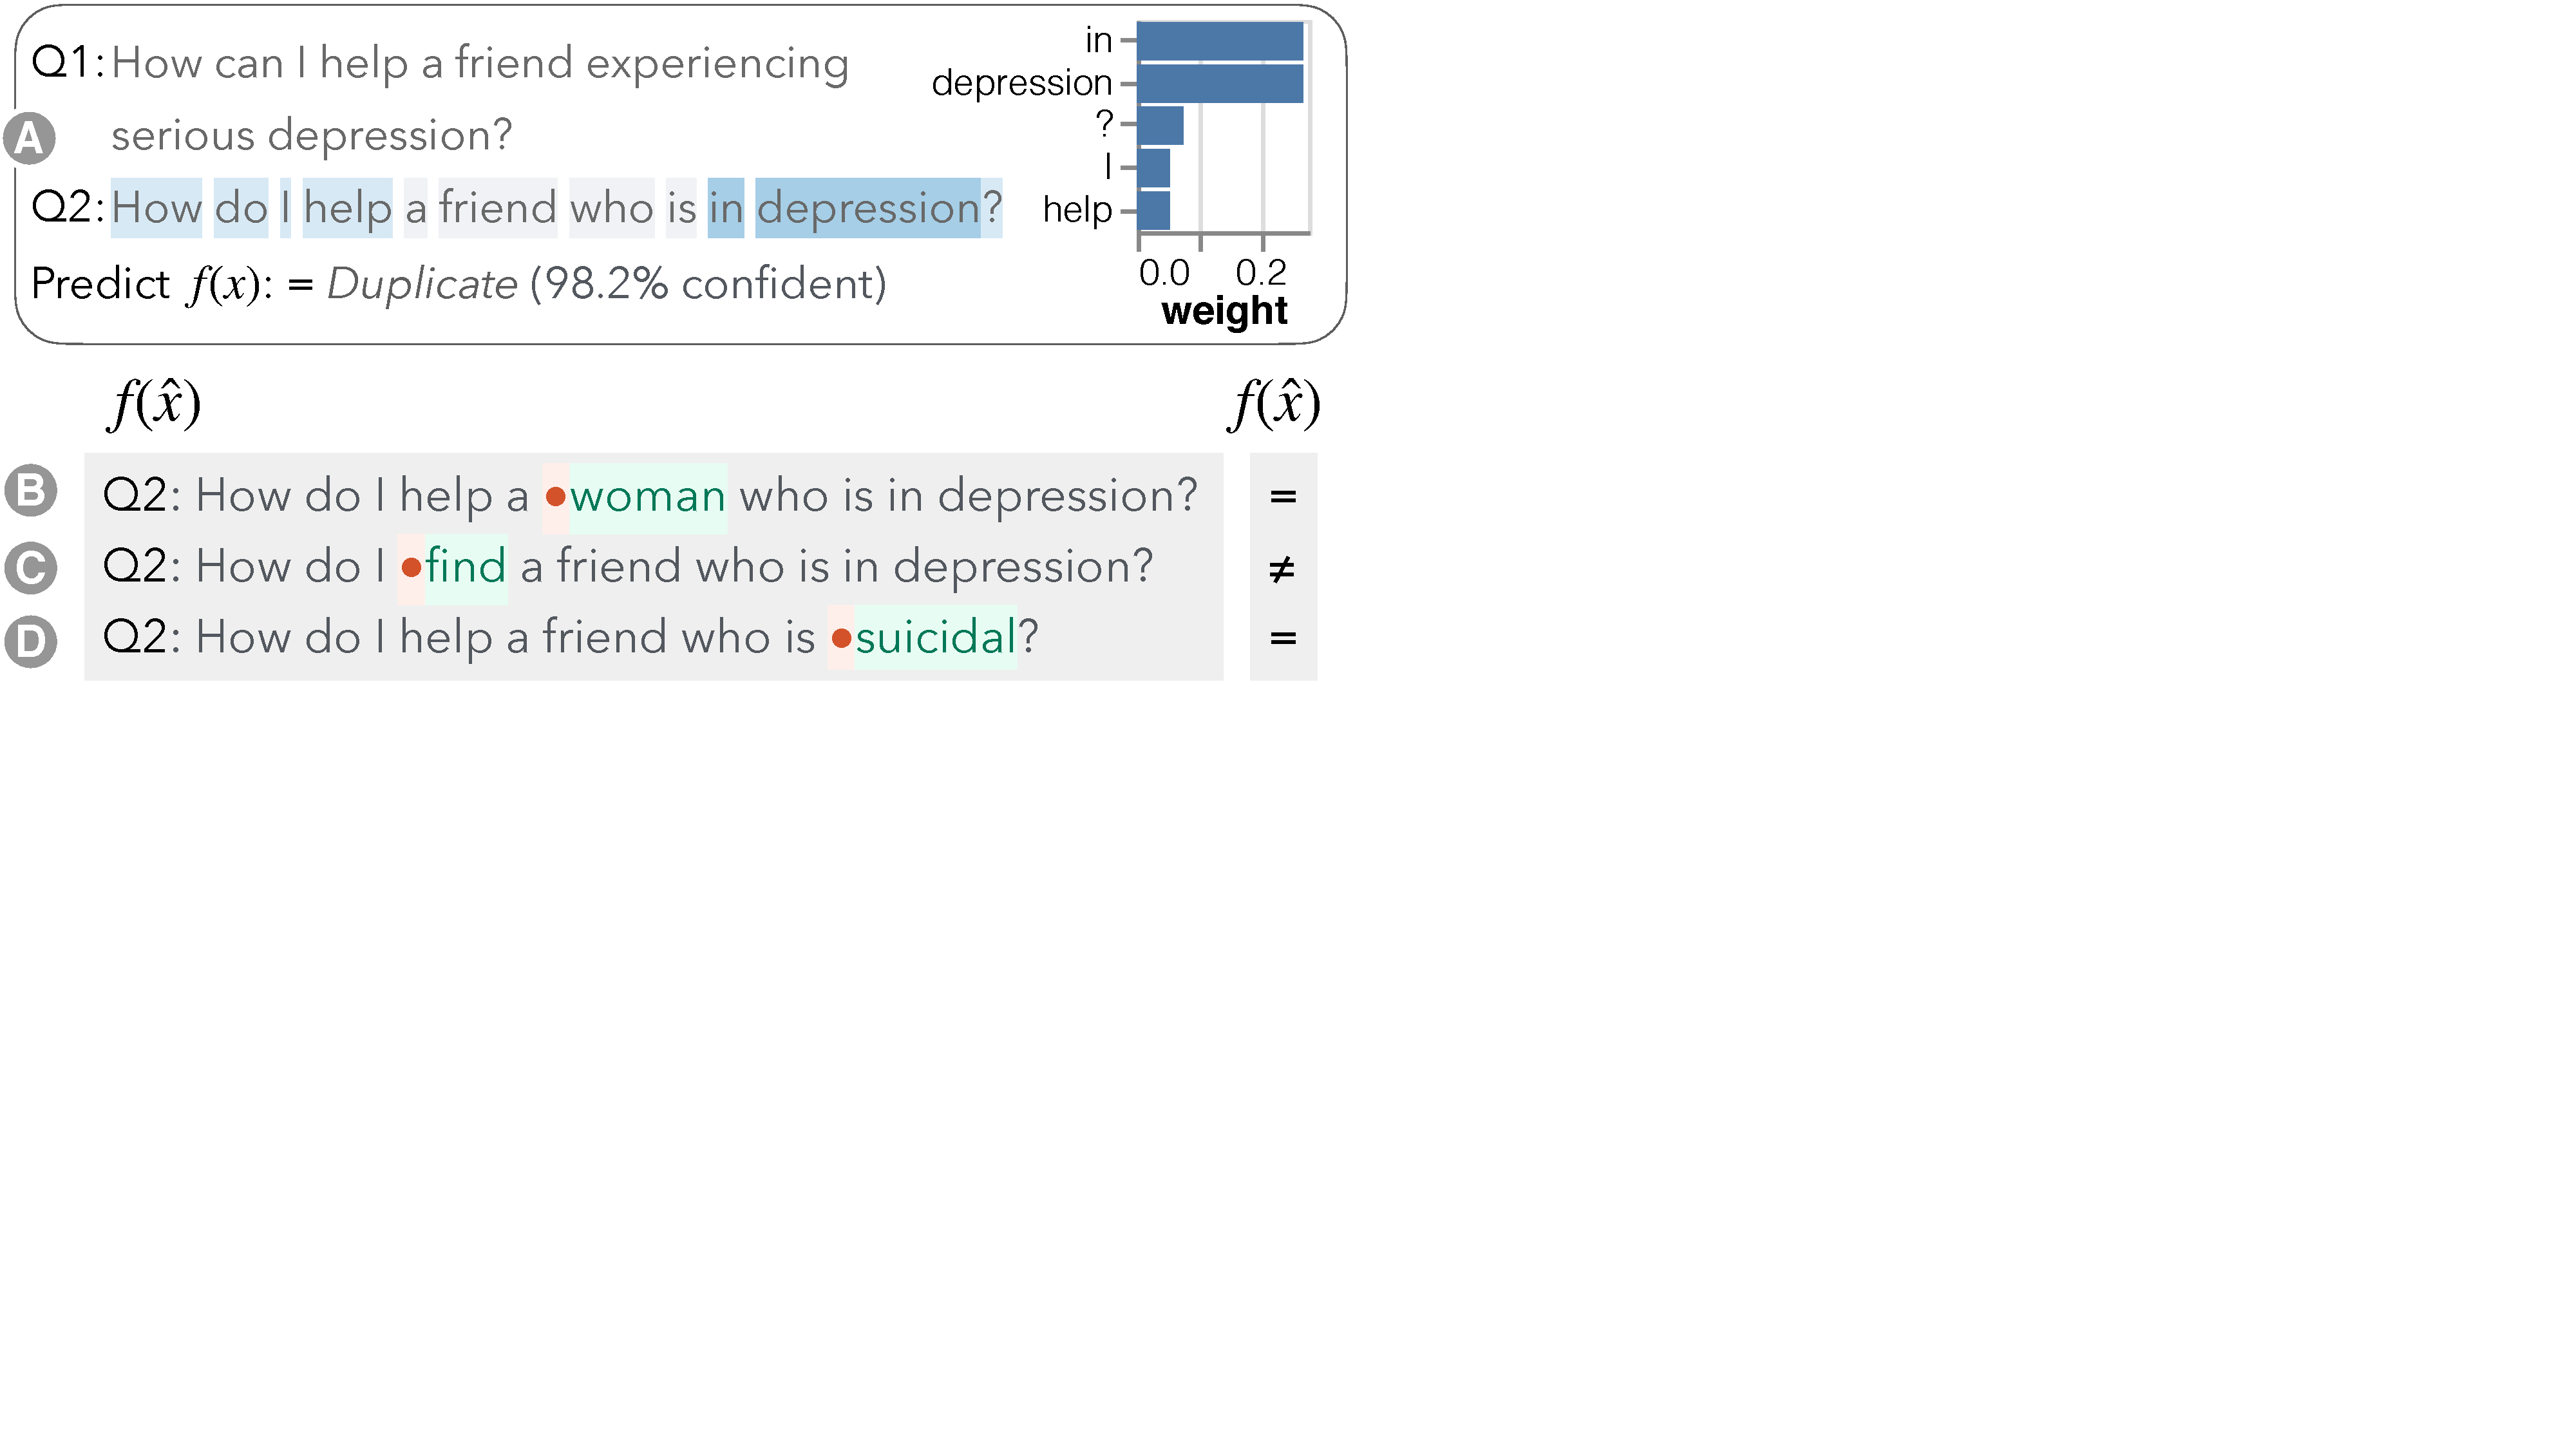
\includegraphics[trim={0 20cm 33cm 0cm},clip,width=1\columnwidth]{figures/explanation_v2}
\vspace{-15pt}
\caption{
(A) A \qqp instance with explanations and predictions ($\mathbf{=}$ means \emph{Duplicate}, $\mathbf{\not\eq}$ \emph{Non-Duplicate}), as well as the feature weights from SHAP.
Counterfactual explanations complement SHAP, \ie they (B) concretize the opaque weights using readable examples, and (C, D) alert abnormalities missed by SHAP.
}
\vspace{-10pt}
\label{fig:explanation}
\end{figure}

%\wts{Finding bugs missed by the feature attribution, and concretizing the opaque weights using readable examples.}
Counterfactual explanations are more intuitive than feature attribution methods~\cite{miller}.
Suppose we are inspecting the \qqp BERT model mentioned in \S\ref{subsec:contrast_set}.
Compared to the opaque SHAP feature weights in Figure~\ref{fig:explanation}A~\cite{NIPS2017_7062}, the concrete example in Figure~\ref{fig:explanation}B more explicitly highlights that the model considers ``help'' trivial (weight$=0.05$): 
\swap{help}{find} in \emph{Q2} does not change the prediction.

However, the cognitive burden of complete explanations around one instance is too great.
As a result, \citet{miller} concluded that people usually \emph{select} a small subset of explanations on contrastive cases (``foils'') that they find unexpected. 
They further proposed that ``abnormality could be used to infer likely foils.''
Here, we operationalize the concept of \emph{abnormality} to select different explanations.


\subsection{Selections for Different Explanations}

\paragraph{Local explanations: expected v.s. actual prediction changes.}
%Compared to feature attribution methods, counterfactual explanations more naturally answer users' 

We define abnormalities around one example as \emph{the discrepancy between the expected and the actual changes in the prediction}.
Given a predictor $f$, we define the actual change in prediction as $d_f(\xp, x)$, and the expected change as $\hat{d}_f(\xp, x)$.
The distance between the expectation and reality then becomes:
$$\Delta d_f(\xp, x) = \hat{d}_f(\xp, x)-d_f(\xp, x)$$
We select two abnormal, ``turning point'' counterfactuals, \ie large gap in prediction when the perturbation is considered trivial: $\xp_l = \argmax_{\xp} \Delta d_f(\xp, x)$, or large perturbation resulting in unchanged prediction: $\xp_s = \argmin_{\xp} \Delta d_f(\xp, x)$.

Whereas $d_f(\xp, x)=|f_p(\xp)-f_p(x)|$ where $f_p(x)$ denotes the prediction probability of $f$ on $x$, $d_f(\xp, x)$ can take various forms. 
As a standalone explanation method, it can be the cosine distance in the \emph{Embedding space}.
The embedding can be either model-agnostic~\cite{reimers-2019-sentence-bert}, or the hidden state of a finetuned predictor.

On the other hand, as a \emph{complement} to existing feature attribution methods, $\hat{d}_f$ can be the importance (weights) of the perturbed tokens in $x$.
Methods like SHAP or LIME provides valuable overview on important features (which is not available in pure counterfactual explanations.
However, as mentioned in \S\ref{sec:relate}, they only estimate weights by \emph{masking} the words, and therefore do not reflect how models would react to replaced words or insertions --- a nuance that is usually overlooked.
Therefore, abnormalities selected this way can help highlight the missed pieces, and better calibrate users' trust on the predictor. 
Figure~\ref{fig:explanation}B shows such a $\xp_l$: \swap{friend}{woman} changes the prediction from \emph{Duplicate} to \emph{Non-Duplicate}, even though ``friend'' is not an important word according to SHAP; Whereas changing the important ``in depression'' in Figure~\ref{fig:explanation}D still results in \emph{Duplicate} ($\xp_s$).
Detailed distance functions are in \S\ref{appendix:exp_rank}.


\paragraph{Interactive explanations: user-selected abnormalities.}
%\paragraph{Interactive explanation.}
Automated selections focus on general abnormality, but users should be able to point towards the part \emph{they} do not understand~\cite{miller}.
%Furthermore, the method should allow explanations as a dialog. 
The targeted generation seamlessly support such interactive explanation.
For example, an analyst can follow up on Figure~\ref{fig:explanation}C, and inspect how the model react to other nouns by blanking ``a friend'' in Q2 (\eg to ``man'' or human names.)


\paragraph{Global Explanations: Recurring edits with unclear impact.}
\label{subsec:global_exp}
%\paragraph{Global explanations: impacts of same changes.}
\emph{Global} explanations provides systematic understandings beyond individual instances --- yet another important aspect of model explanations~\cite{miller}.
We define global abnormality as \emph{perturbation patterns whose impacts on the prediction are hard to generalize}, and find them in two steps:
First, we featurize counterfactuals to create groups of similar counterfactuals, using the \tagstr between $\xp$ and $x$, the edited spans, etc.
%(1) its \tagstr (\fexptag{negation} for the example in Figure~\ref{fig:blank}), 
%(2) its remove phrases \fexpfrom{kids}, 
%(3) its added phrases \fexpto{not}, \fexpto{children}, and 
%(4) the combined template \fexptemp{\swap{kids}{children}}.
Then, we rank the groups using the entropy of the prediction changes $(f(x) \rightarrow f(\xp))$ for all counterfactuals in a group.
Larger entropy indicates that the perturbation has unstable impact on the prediction.

For example, when evaluating the \nli RoBERTa model (the same as in \S\ref{subsec:contrast_set}), one abnormal global perturbation is \swap{two}{three} in the hypothesis.
Out of the 253 counterfactuals whose original $f(x)=$ \emph{entailment}, $138$ flipped to \emph{contradiction}, $22$ to \emph{neutral}, yet $93$ remained \emph{entailment}, resulting in entropy $I=0.91$.
We observe that most cases flipped to \emph{contradiction} have the explicit word ``two'' in the premise, whereas the prediction-intact ones suggest that the model struggles with counting:

\ebox{
\textbf{P}: Two women having drinks at the bar.\\
\textbf{H}: \swap{Two}{Three} women are at a bar.\\
\textbf{$\mathbf{f(x)\rightarrow f(\xp)}$}: \swap{entailment}{contradiction}\\
--\\
\textbf{P}: A boy and a girl gaze in a clothing store window.\\
\textbf{H}: \swap{Two}{Three} kids are looking in a store window.\\
\textbf{$\mathbf{f(x)\rightarrow f(\xp)}$}: \swap{entailment}{entailment}
}


\subsection{Local Exp.: Complement SHAP?}
\label{subsec:exp_user_study}

We conduct a user study to verify whether our local counterfactual explanations can complement SHAP, as the setup nicely combines the overview provided by SHAP, and the decision boundaries it omits.
%\footnote{We defer more sophisticated designs and evaluations for interactive and global explanation to future work.}
%, where participants are asked to predict model's behavior on the given variations of a base example.
The study takes the form of counterfactual simulation~\cite{hase2020evaluating}, with participants predicting a model's behavior on counterfactuals.
Intuitively, the more they simulate incorrectly, the more information they grasp \emph{if we show the counterfactuals to them}.

\paragraph{Procedure.}
We recruited \tofix{13} graduate students who have intermediate NLP knowledge and have experience using model explanations, and asked them to simulate the behavior of a \qqp BERT model for 20 rounds.
In each round, the participants were given a base example with the model's prediction, as well as the SHAP weights, highlighted in the text and with a bar chart (Figure~\ref{fig:explanation}A).
The participants were allowed to 

query the model around the base example for up to 10 times, by making small changes to Q2 and seeing the resulting model predictions.
It was equivalent to unlimited model access --- participants submitted $6.3\pm3.2$ queries per round.
More interactions with the predictor usually result in better mental models~\cite{miller}, and we are interested in whether our selected ones \emph{still add information} afterwards.
Participants then simulated the model's predictions on six counterfactuals (displayed similar to Figure~\ref{fig:explanation}B), two from each of the following three conditions.
We concluded the study with open-ended questions on their model query and simulation strategies.



\newcommand{\cshap}{\emph{SHAP-c}\xspace}
\newcommand{\crandom}{\emph{Random}\xspace}
\newcommand{\chuman}{\emph{Human}\xspace}
\paragraph{Conditions.} 
We compare three types of counterfactuals:
(1) \cshap, the \sysname-generated counterfactuals, selected to complement SHAP; 
(2) \crandom, the randomly selected \sysname counterfactuals; 
(3) \chuman, the human generated counterfactuals.
For every base example, three graduate students each queried the model for up to 10 times and submitted one counterfactual, where the model prediction was incorrect and counterintuitive with respect to the original SHAP score.
We then randomly selected two of their submissions per base example.




\begin{figure}[t]
\centering
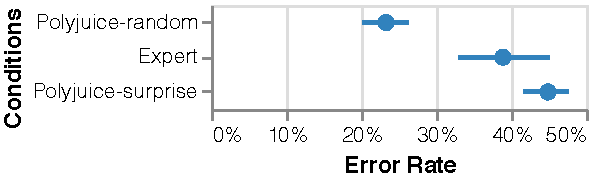
\includegraphics[width=1\columnwidth]{figures/err_rate}
\vspace{-15pt}
\caption{
Error rates on counterfactuals in different conditions. The higher the error rate, the more information missed by the participants (\ie and therefore can better complement model interactions and SHAP.)
}
\vspace{-10pt}
\label{fig:err_rate}
\end{figure}

\paragraph{Results.}
As a within-subject study, we compared \emph{the error rate of human simulations across the three conditions}.
Figure~\ref{fig:err_rate} shows that, compared to \crandom (error rate $e=23\%\pm6\%$) and \chuman ($e=38\%\pm11\%$), participants mis-simulated more \cshap counterfactuals ($45\%\pm 6\%$).
While they were able to simulate model behaviors on some counterfactuals, \cshap ones were beyond their learnings from SHAP and model interactions, and \emph{would still add value if they were presented.}


More interestingly, \emph{\cshap found more bugs within spots where humans considered inspected.}
Usually, participants simulated the model incorrectly because they missed the inspection spots.
For example, they focused on editing ``depression'' in Figure~\ref{fig:explanation}A, and therefore had to ``guess using intuitions'' when simulating Figure~\ref{fig:explanation}B.
However, in 24\% of the missed \cshap cases, users successfully covered the related pattern\footnote{At least one of their queries perturbed the same spans as the given counterfactual, and the text overlap between the query and the counterfactual is over 70\%}, and was misled by their inspections --- ``labeled based on similar examples I tried'', as one subject articulated.
It was hard for them to imagine model predicting \emph{Duplicate} on Figure~\ref{fig:explanation}B (\swap{help}{find}), when the model predicted \emph{Non-Duplicate} on their query \exinline{How do I \swap{help}{play with}...?}
The number dropped to $15\%$ for the \chuman condition.


Moreover, in their freeform responses, 7 out of 13 participants mentioned they prioritized perturbing words with high feature weights, further indicating the importance of selecting \emph{unexpected prediction change} for them.


